% Sketch output, version 0.2 (build 161, Tue Sep 8 23:35:27 2009)
% Output language: PGF/TikZ,LaTeX
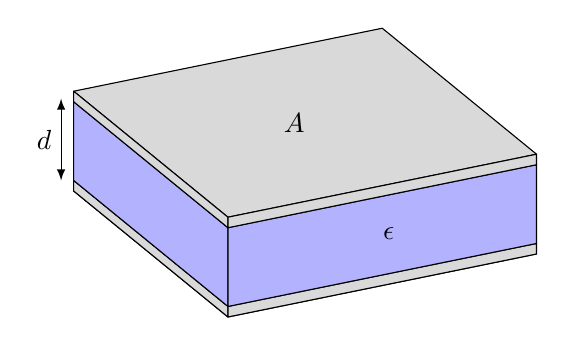
\begin{tikzpicture}[line join=round,scale=0.8]
\filldraw[fill=gray!30](2.449,-2.167)--(7.348,-1.167)--(4.899,.833)--(0,-.167)--cycle;
\filldraw[fill=gray!30](2.449,-2)--(7.348,-1)--(4.899,1)--(0,0)--cycle;
\filldraw[fill=blue!30](2.449,-2)--(7.348,-1)--(4.899,1)--(0,0)--cycle;
\filldraw[fill=gray!30](2.449,-.75)--(7.348,.25)--(4.899,2.25)--(0,1.25)--cycle;
\filldraw[fill=blue!30](2.449,-.75)--(7.348,.25)--(4.899,2.25)--(0,1.25)--cycle;
\filldraw[fill=gray!30](2.449,-.583)--(7.348,.417)--(4.899,2.417)--(0,1.417)--cycle;
\filldraw[fill=gray!30](0,-.167)--(2.449,-2.167)--(2.449,-2)--(0,0)--cycle;
\filldraw[fill=blue!30](0,0)--(2.449,-2)--(2.449,-.75)--(0,1.25)--cycle;
\filldraw[fill=gray!30](0,1.25)--(2.449,-.75)--(2.449,-.583)--(0,1.417)--cycle;
\filldraw[fill=gray!30](2.449,-2.167)--(7.348,-1.167)--(7.348,-1)--(2.449,-2)--cycle;
\filldraw[fill=blue!30](2.449,-2)--(7.348,-1)--(7.348,.25)--(2.449,-.75)--cycle;
\filldraw[fill=gray!30](2.449,-.75)--(7.348,.25)--(7.348,.417)--(2.449,-.583)--cycle;
\draw[<->,>=latex] (-0.2,0) -- node[left] {$d$} (-0.2,1.3);
\node [right=0.8*5cm,below=0.8*0.6cm] {$\epsilon$};
\node [right=0.8*3.5cm,above=0.8*0.6cm] {$A$};
\end{tikzpicture}% End sketch output
